%%=============================================================================
%% Proof-of-concept: Conventioneel
%%=============================================================================

\chapter{\IfLanguageName{dutch}{Proof-of-concept: Conventioneel}{Proof-of-concept: Conventional}}%
\label{ch:proofofconceptConventioneel}

\section{Inleiding}

In dit hoofdstuk zal een overzicht gegeven worden over hoe de conventionele webshop is opgebouwd. Hier zal echter niet dieper ingaan op het technische aspect van de React componenten of de API-calls die gerealiseerd zijn.

\section{Mock-ups}

Alvorens er een lijn code geschreven wordt zijn er mock-ups gemaakt voor de mobiele versie \ref{fig:mobileMockUps} en de desktop versie, beide voor de Home Pagina \ref{fig:desktopHomeMockUp} en de Detail Pagina \ref{fig:desktopDetailMockUp}. Zoals eerder vermeld dienen de mock-ups als een basis voor de conventionele versie van de webshop om een goede UX/UI te voorzien.

\begin{figure}
	\centering
	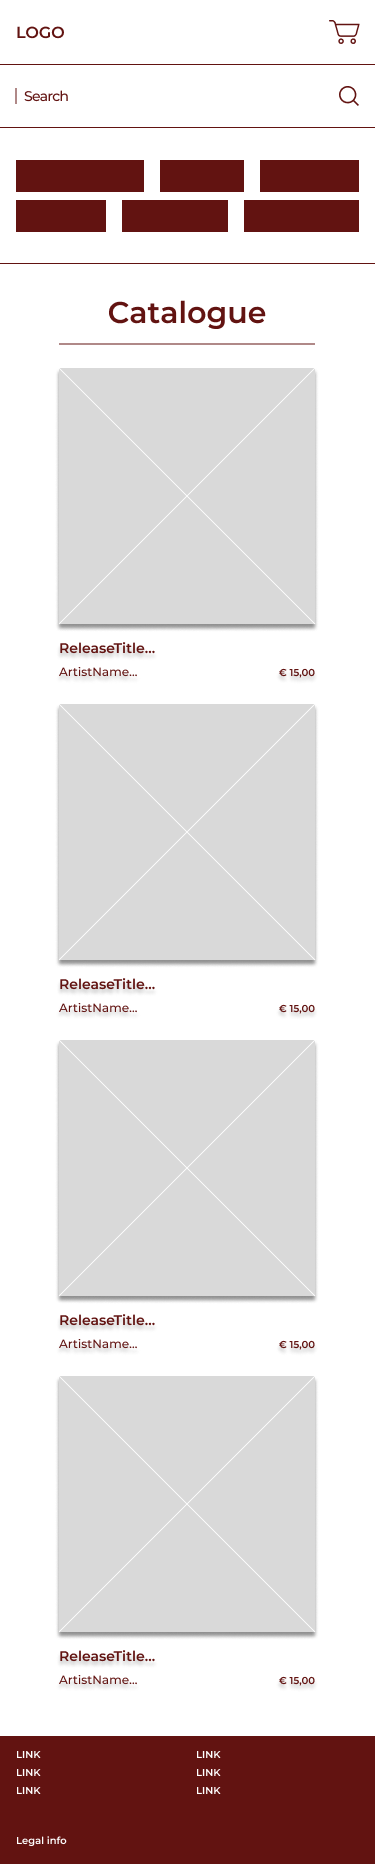
\includegraphics[width=0.3\linewidth]{graphics/HomePageMobile}
	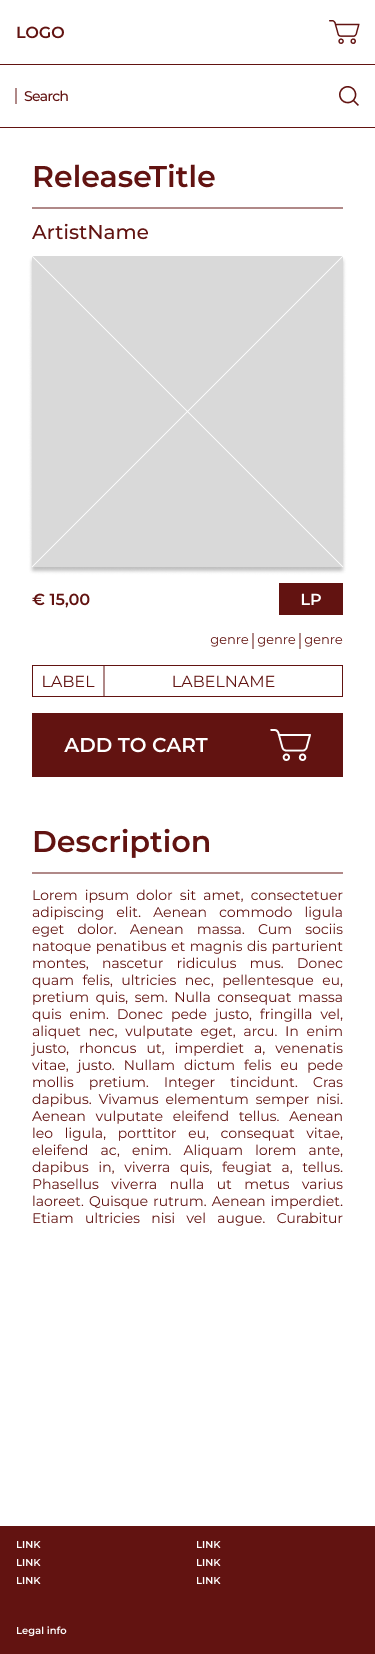
\includegraphics[width=0.3\linewidth]{graphics/DetailsPageMobile}
	\caption[Mock-Ups Mobile]{Mock-Ups Mobile}
	\label{fig:mobileMockUps}
\end{figure}

\begin{figure}
	\centering
	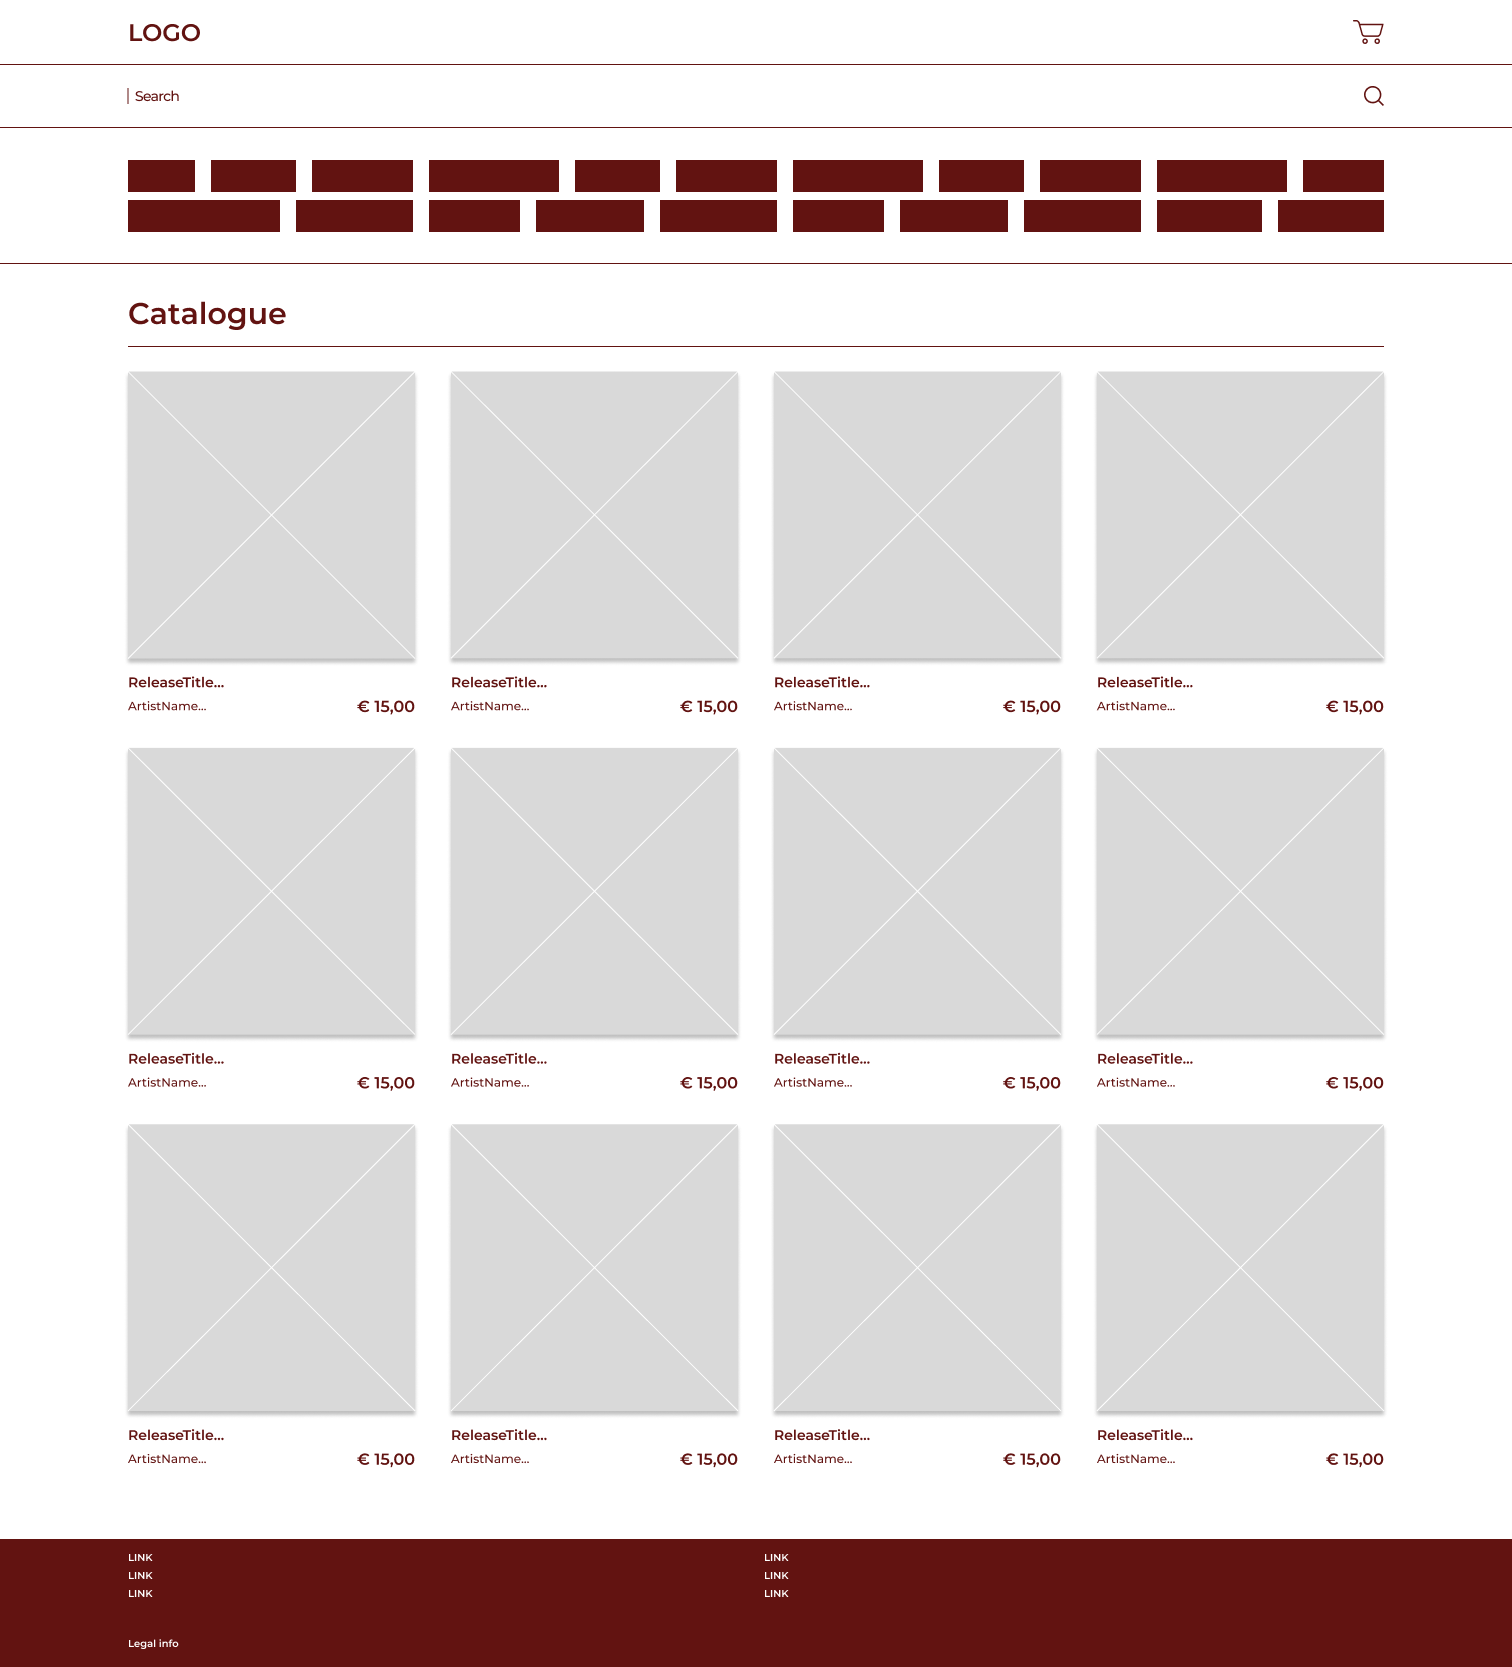
\includegraphics[width=1\linewidth]{graphics/HomePageDesktop}
	\caption[Mock-Up Desktop]{Mock-Up Desktop Home Pagina}
	\label{fig:desktopHomeMockUp}
\end{figure}

\begin{figure}
	\centering
	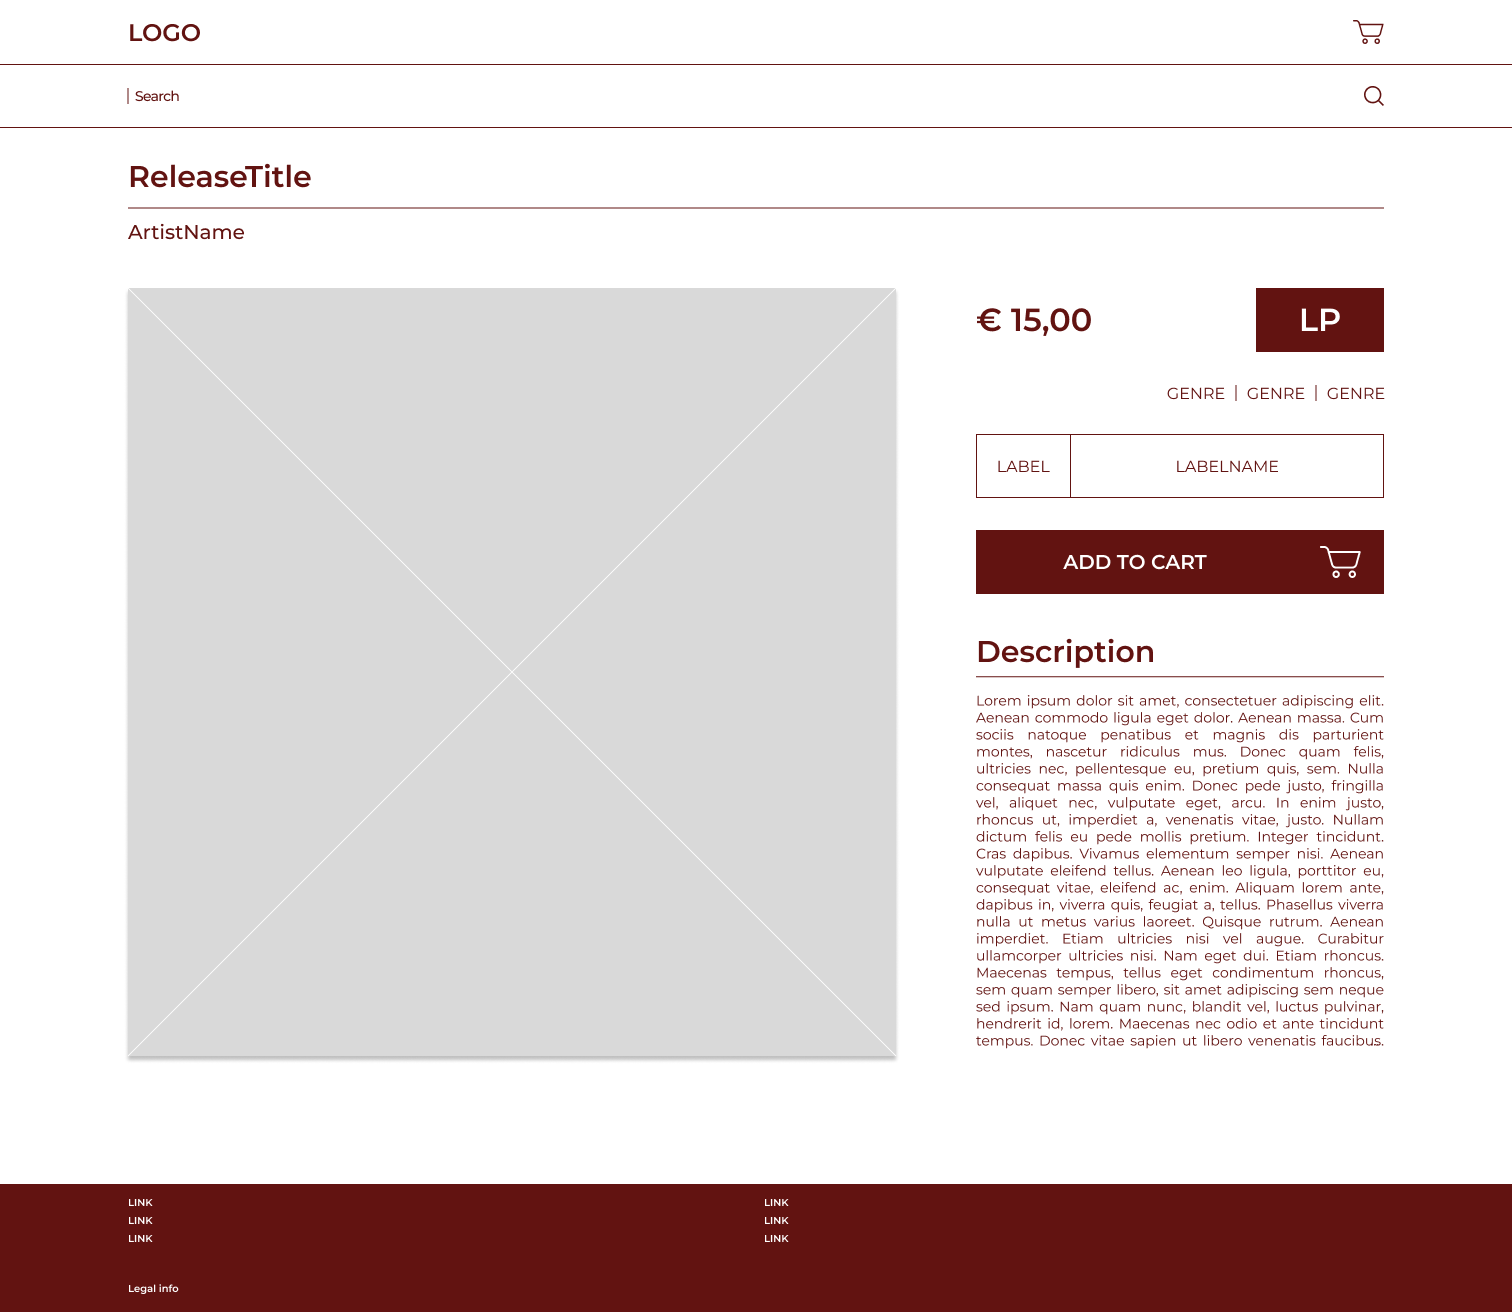
\includegraphics[width=1\linewidth]{graphics/DetailPageDesktop}
	\caption[Mock-Up Desktop]{Mock-Up Desktop Detail Pagina}
	\label{fig:desktopDetailMockUp}
\end{figure}

\pagebreak

\section{Home pagina}

De opbouw van de home pagina is als volgt. Wanneer men de conventionele webshop opent dan krijgt men een Trending pagina te zien, deze is gebaseerd op de nieuwste releases van Spotify. Als de gebruiker klikt op een ReleaseItem dan wordt hij/zij verwezen naar de Detail pagina van deze release. De gebruiker kan ook op "Show More" klikken indien hij/zij meer dan 8 releases wil zien. Zie figuur \ref{fig:desktopHomeConventioneel} voor een beeld van de home pagina.

\begin{figure}
	\centering
	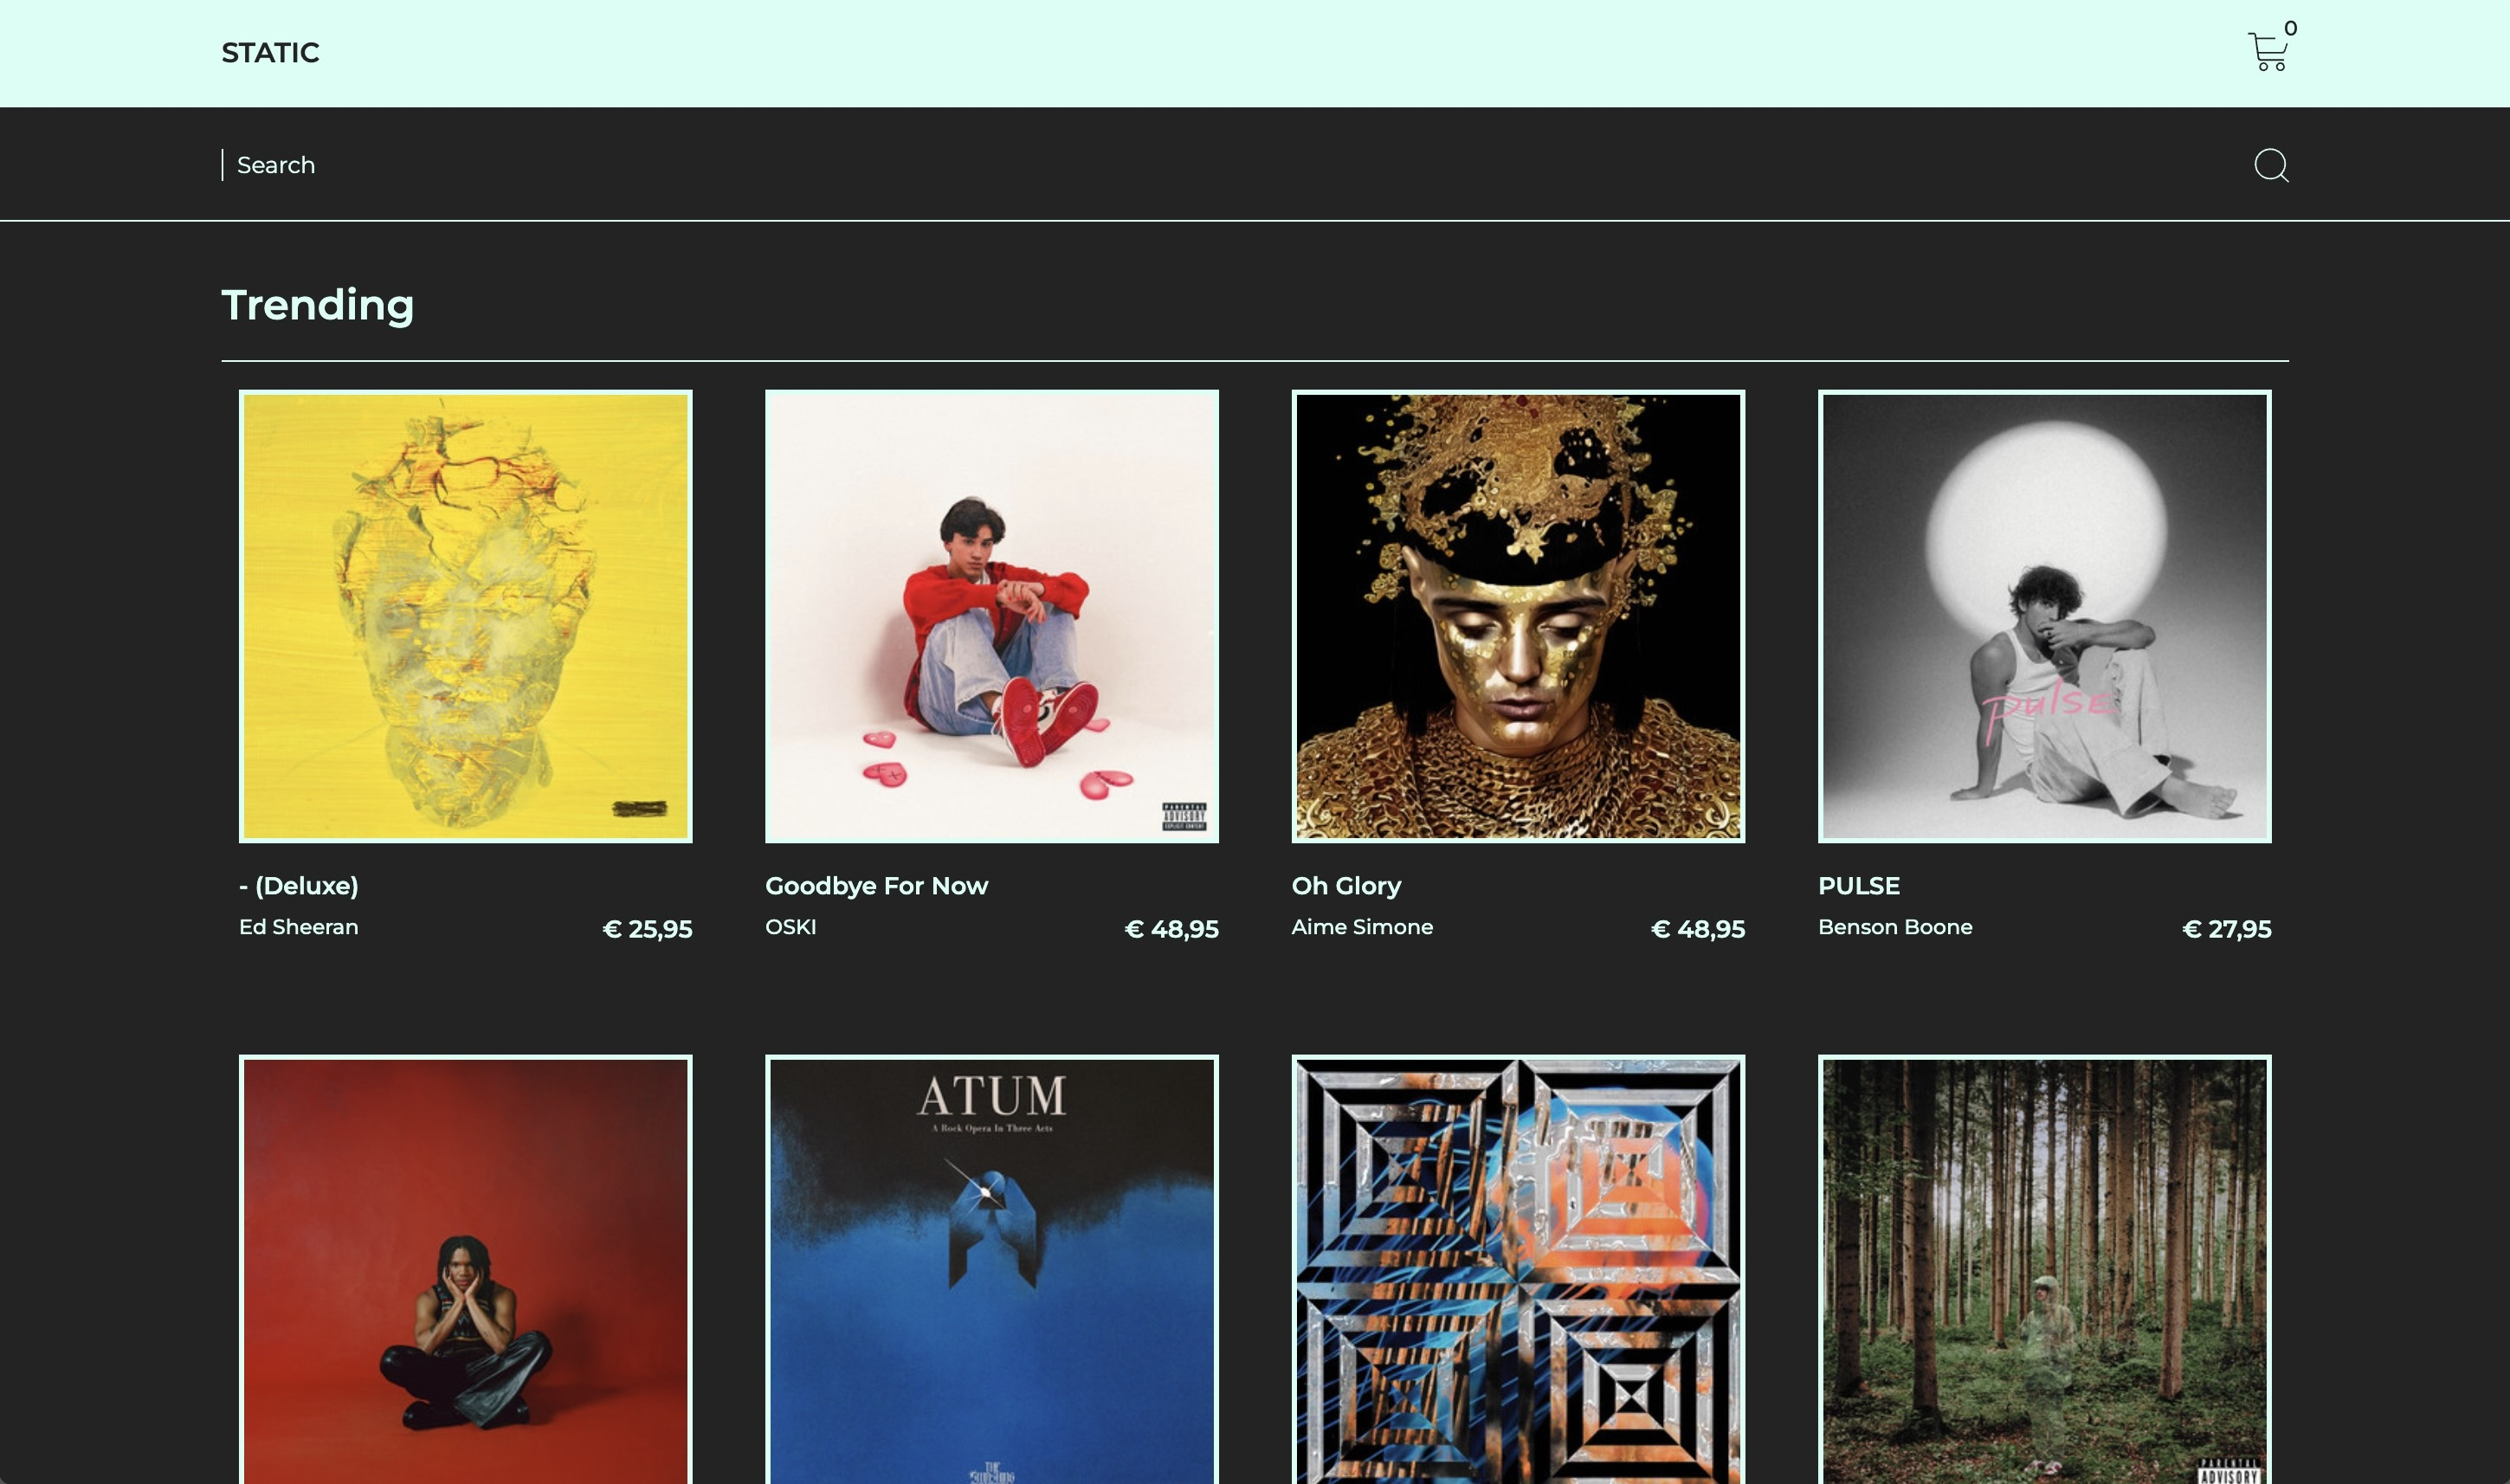
\includegraphics[width=1\linewidth]{graphics/desktopHomeConventioneel}
	\caption[Desktop home pagina conventioneel]{Desktop home pagina conventioneel}
	\label{fig:desktopHomeConventioneel}
\end{figure}

\section{Detail pagina}

Wanneer de gebruiker zich op de Detail pagina bevindt krijgt hij/zij alle details te zien van de release. Waaronder de prijs, de releasedatum, het label en alle liedjes die behoren tot de release. De gebruiker heeft twee opties. Met de "ADD TO CART" knop kan men een release toevoegen aan de winkelmand of men kan ook doorverwezen worden naar Spotify om daar de release te beluisteren. Hier heeft men ook de mogelijkheid om naar een andere release te zoeken a.d.h.v. de zoekbalk. Als men een release toevoegt aan de winkelmand dan krijgt de gebruiker een pop-up ter bevestiging. Zie figuur \ref{fig:desktopDetailConventioneel} voor een beeld van de home pagina.

\begin{figure}
	\centering
	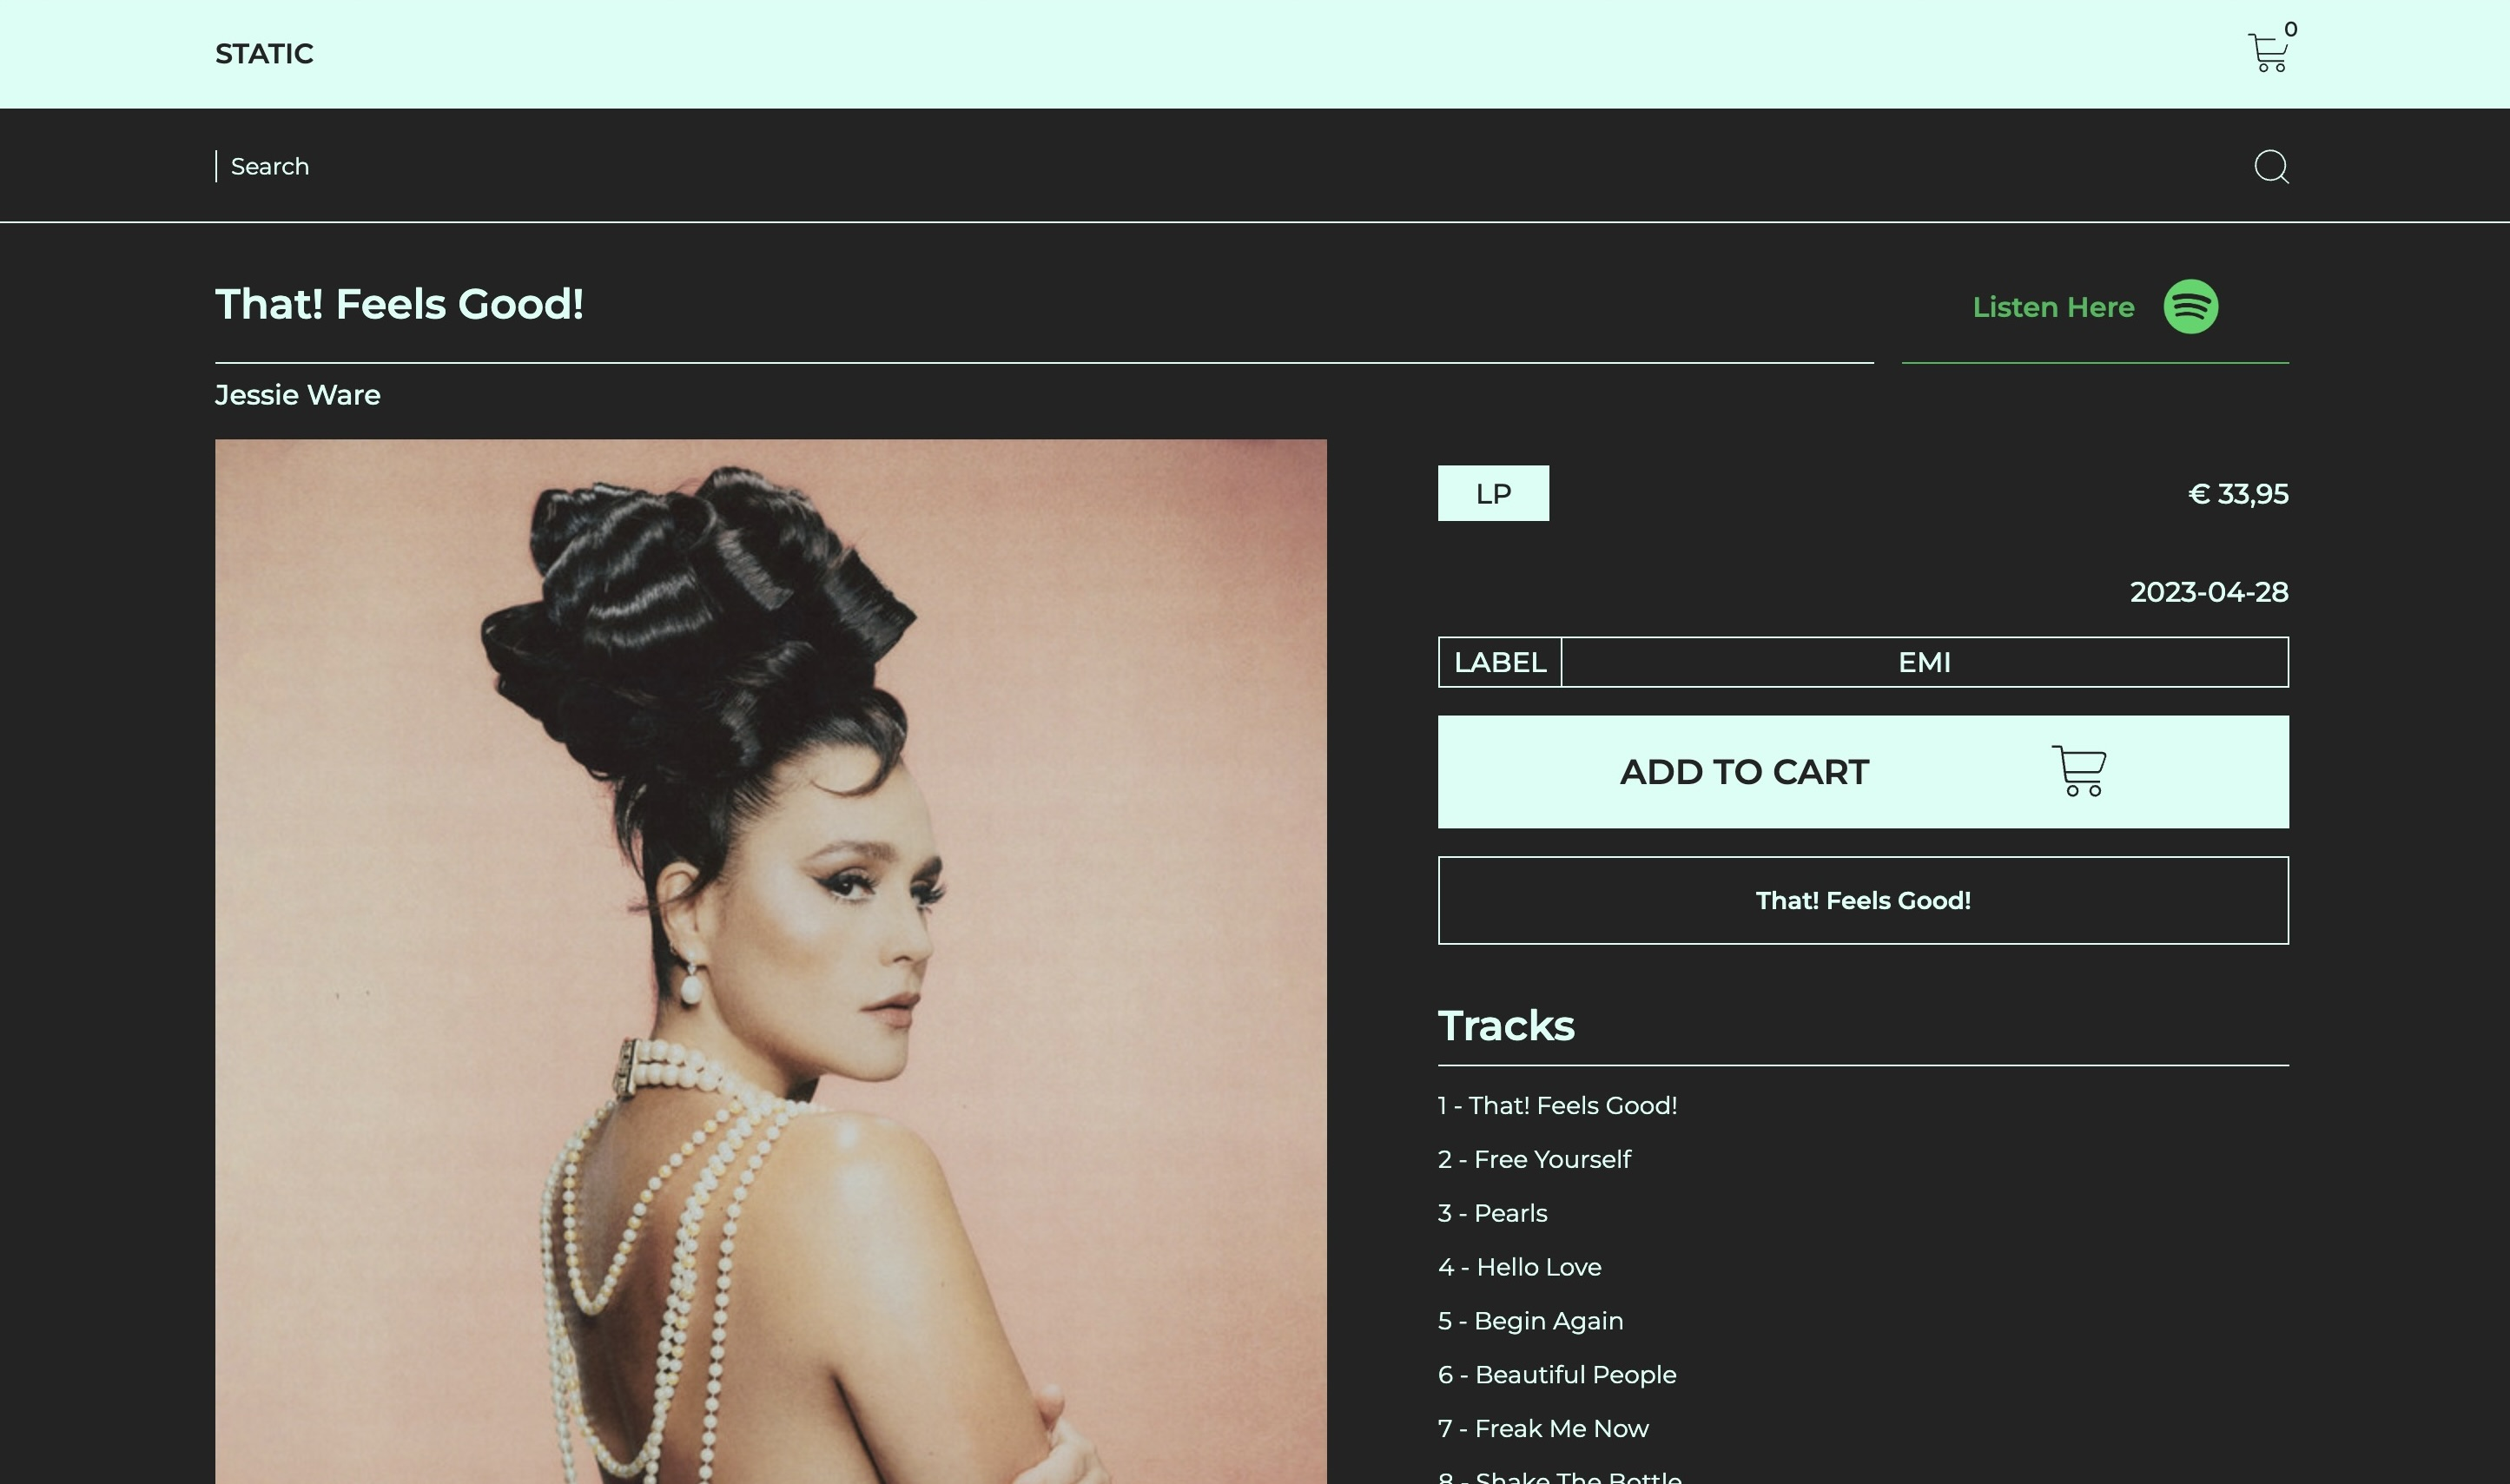
\includegraphics[width=1\linewidth]{graphics/desktopDetailConventioneel}
	\caption[Desktop detail pagina conventioneel]{Desktop detail pagina conventioneel}
	\label{fig:desktopDetailConventioneel}
\end{figure}

\section{Cart}

Nu kan de gebruiker de geselecteerde releases bekijken in de winkelmand door in de header op het winkelmand icoon te klikken. Hier krijgt men een overzicht en kan men indien gewenst de hoeveelheid aanpassen of releases verwijderen. Zie figuur \ref{fig:desktopCart} voor een beeld van de home pagina.

\begin{figure}
	\centering
	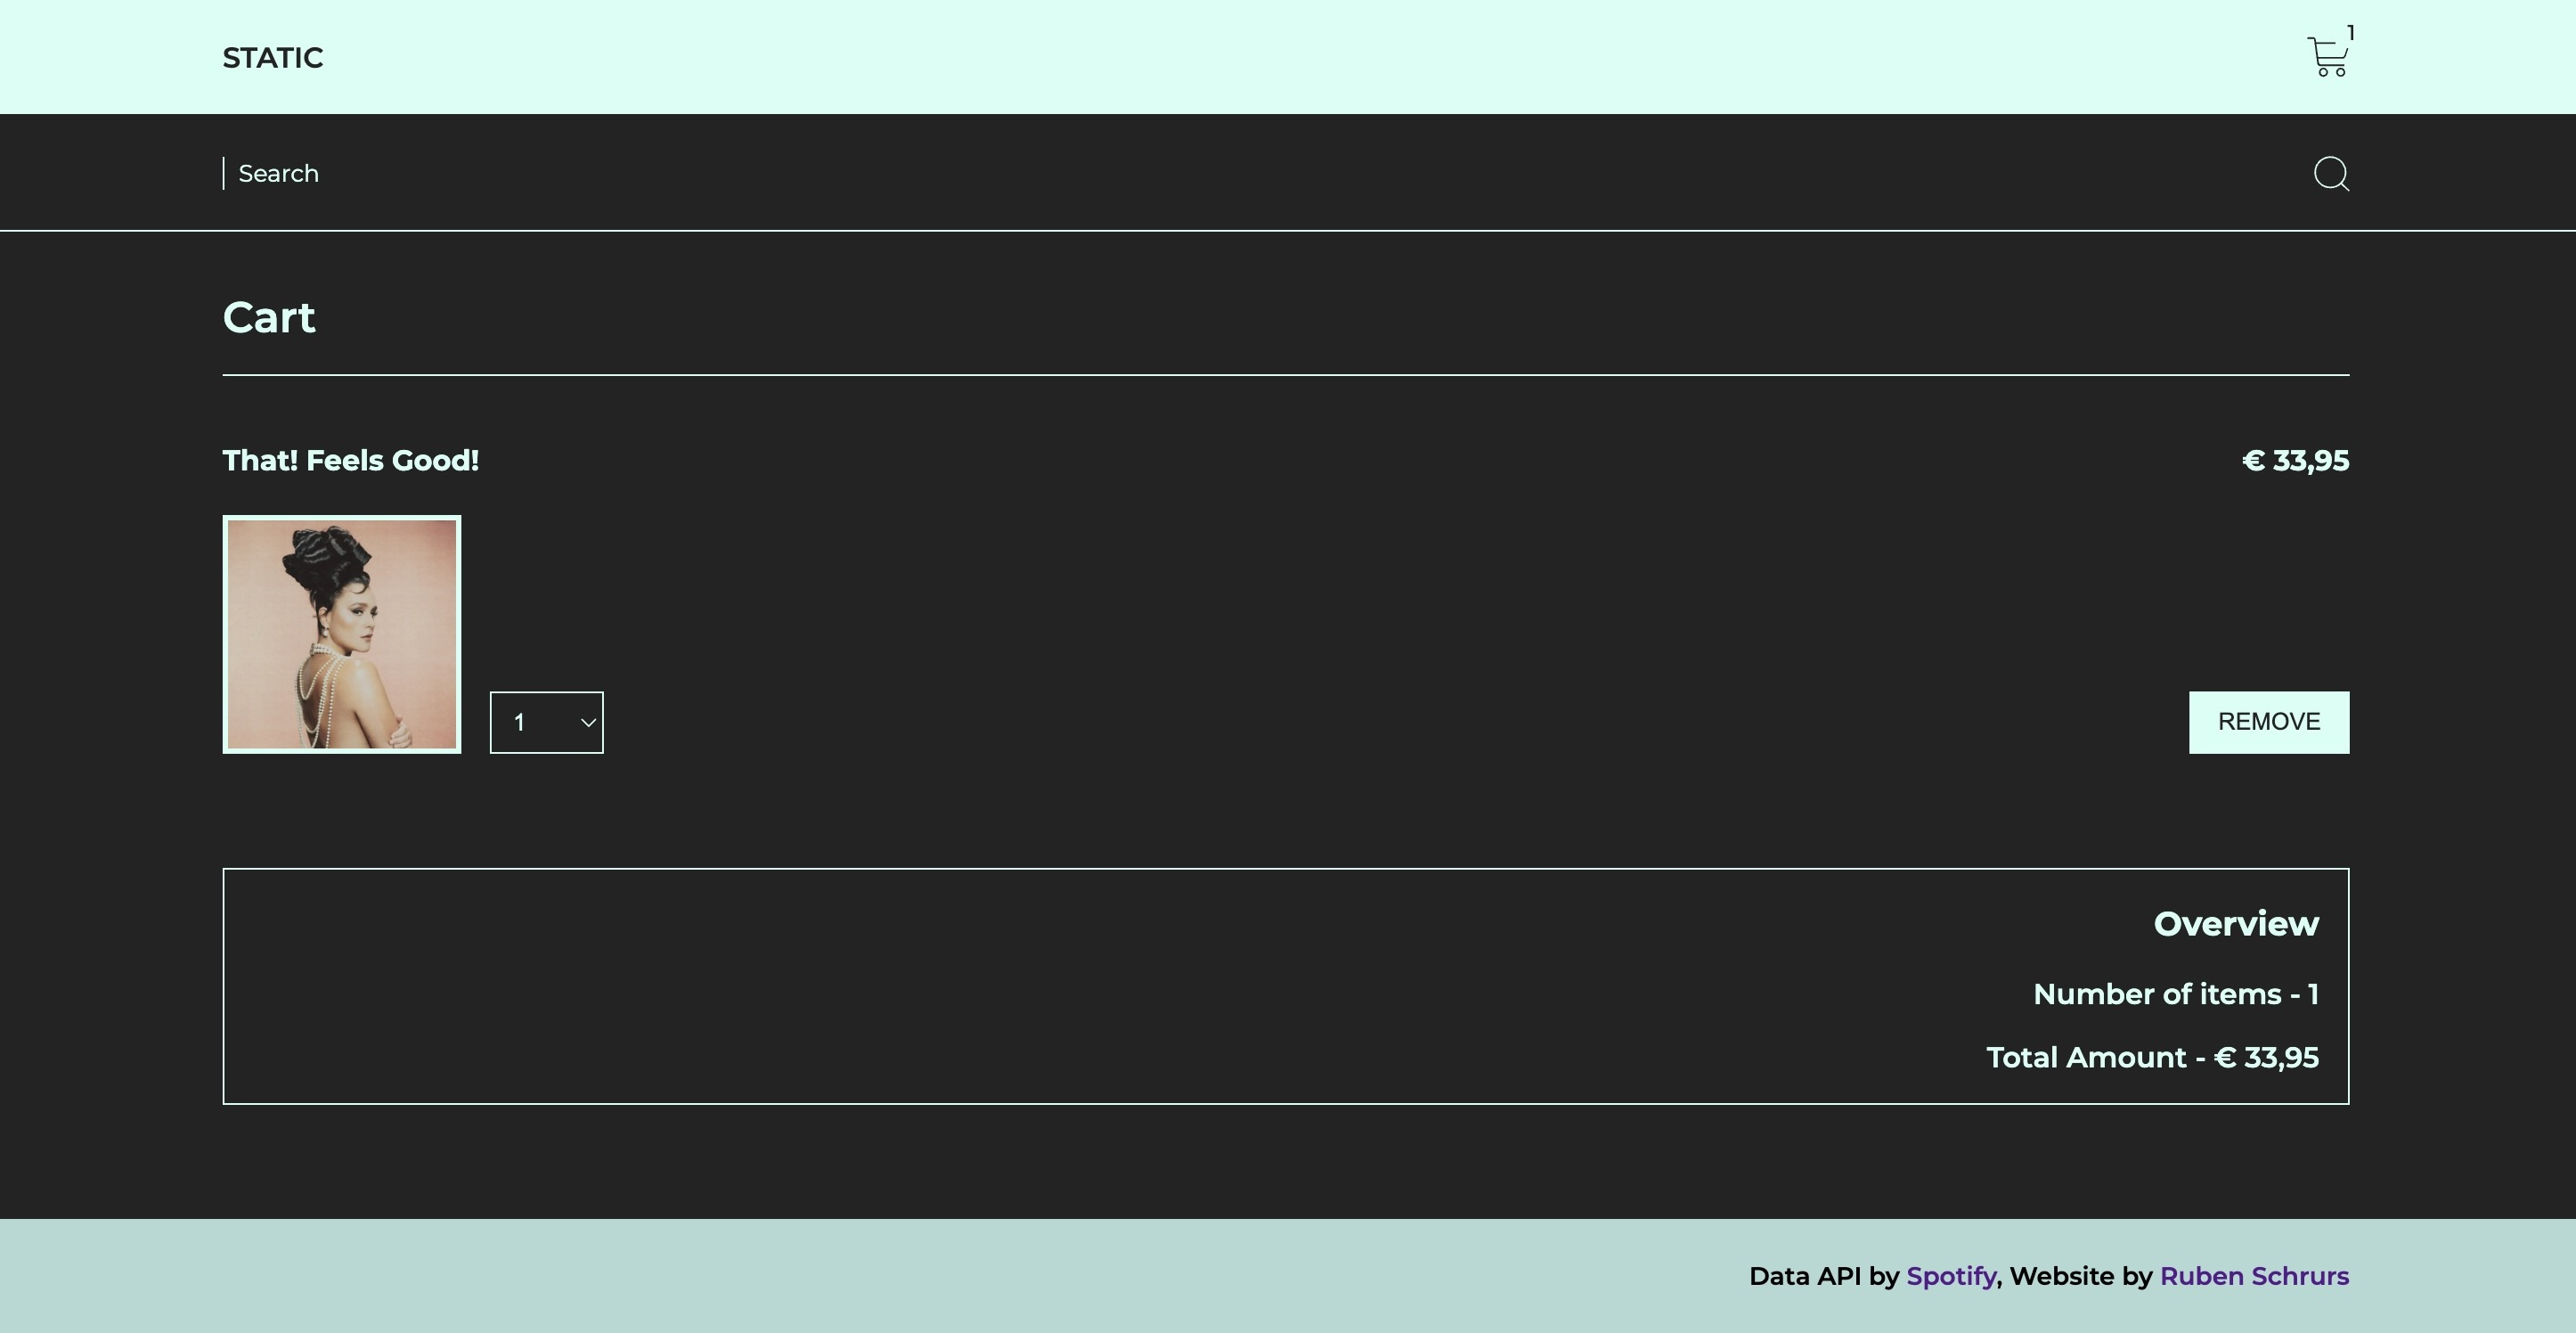
\includegraphics[width=1\linewidth]{graphics/desktopCart}
	\caption[Desktop cart pagina]{Desktop cart pagina}
	\label{fig:desktopCart}
\end{figure}

\section{Search}

Onder de header bevindt zich de search bar, deze kan de gebruiker over de volledige website gebruiken en zal volgend resultaat opleveren, zie figuur \ref{fig:desktopSearch}.

\begin{figure}
	\centering
	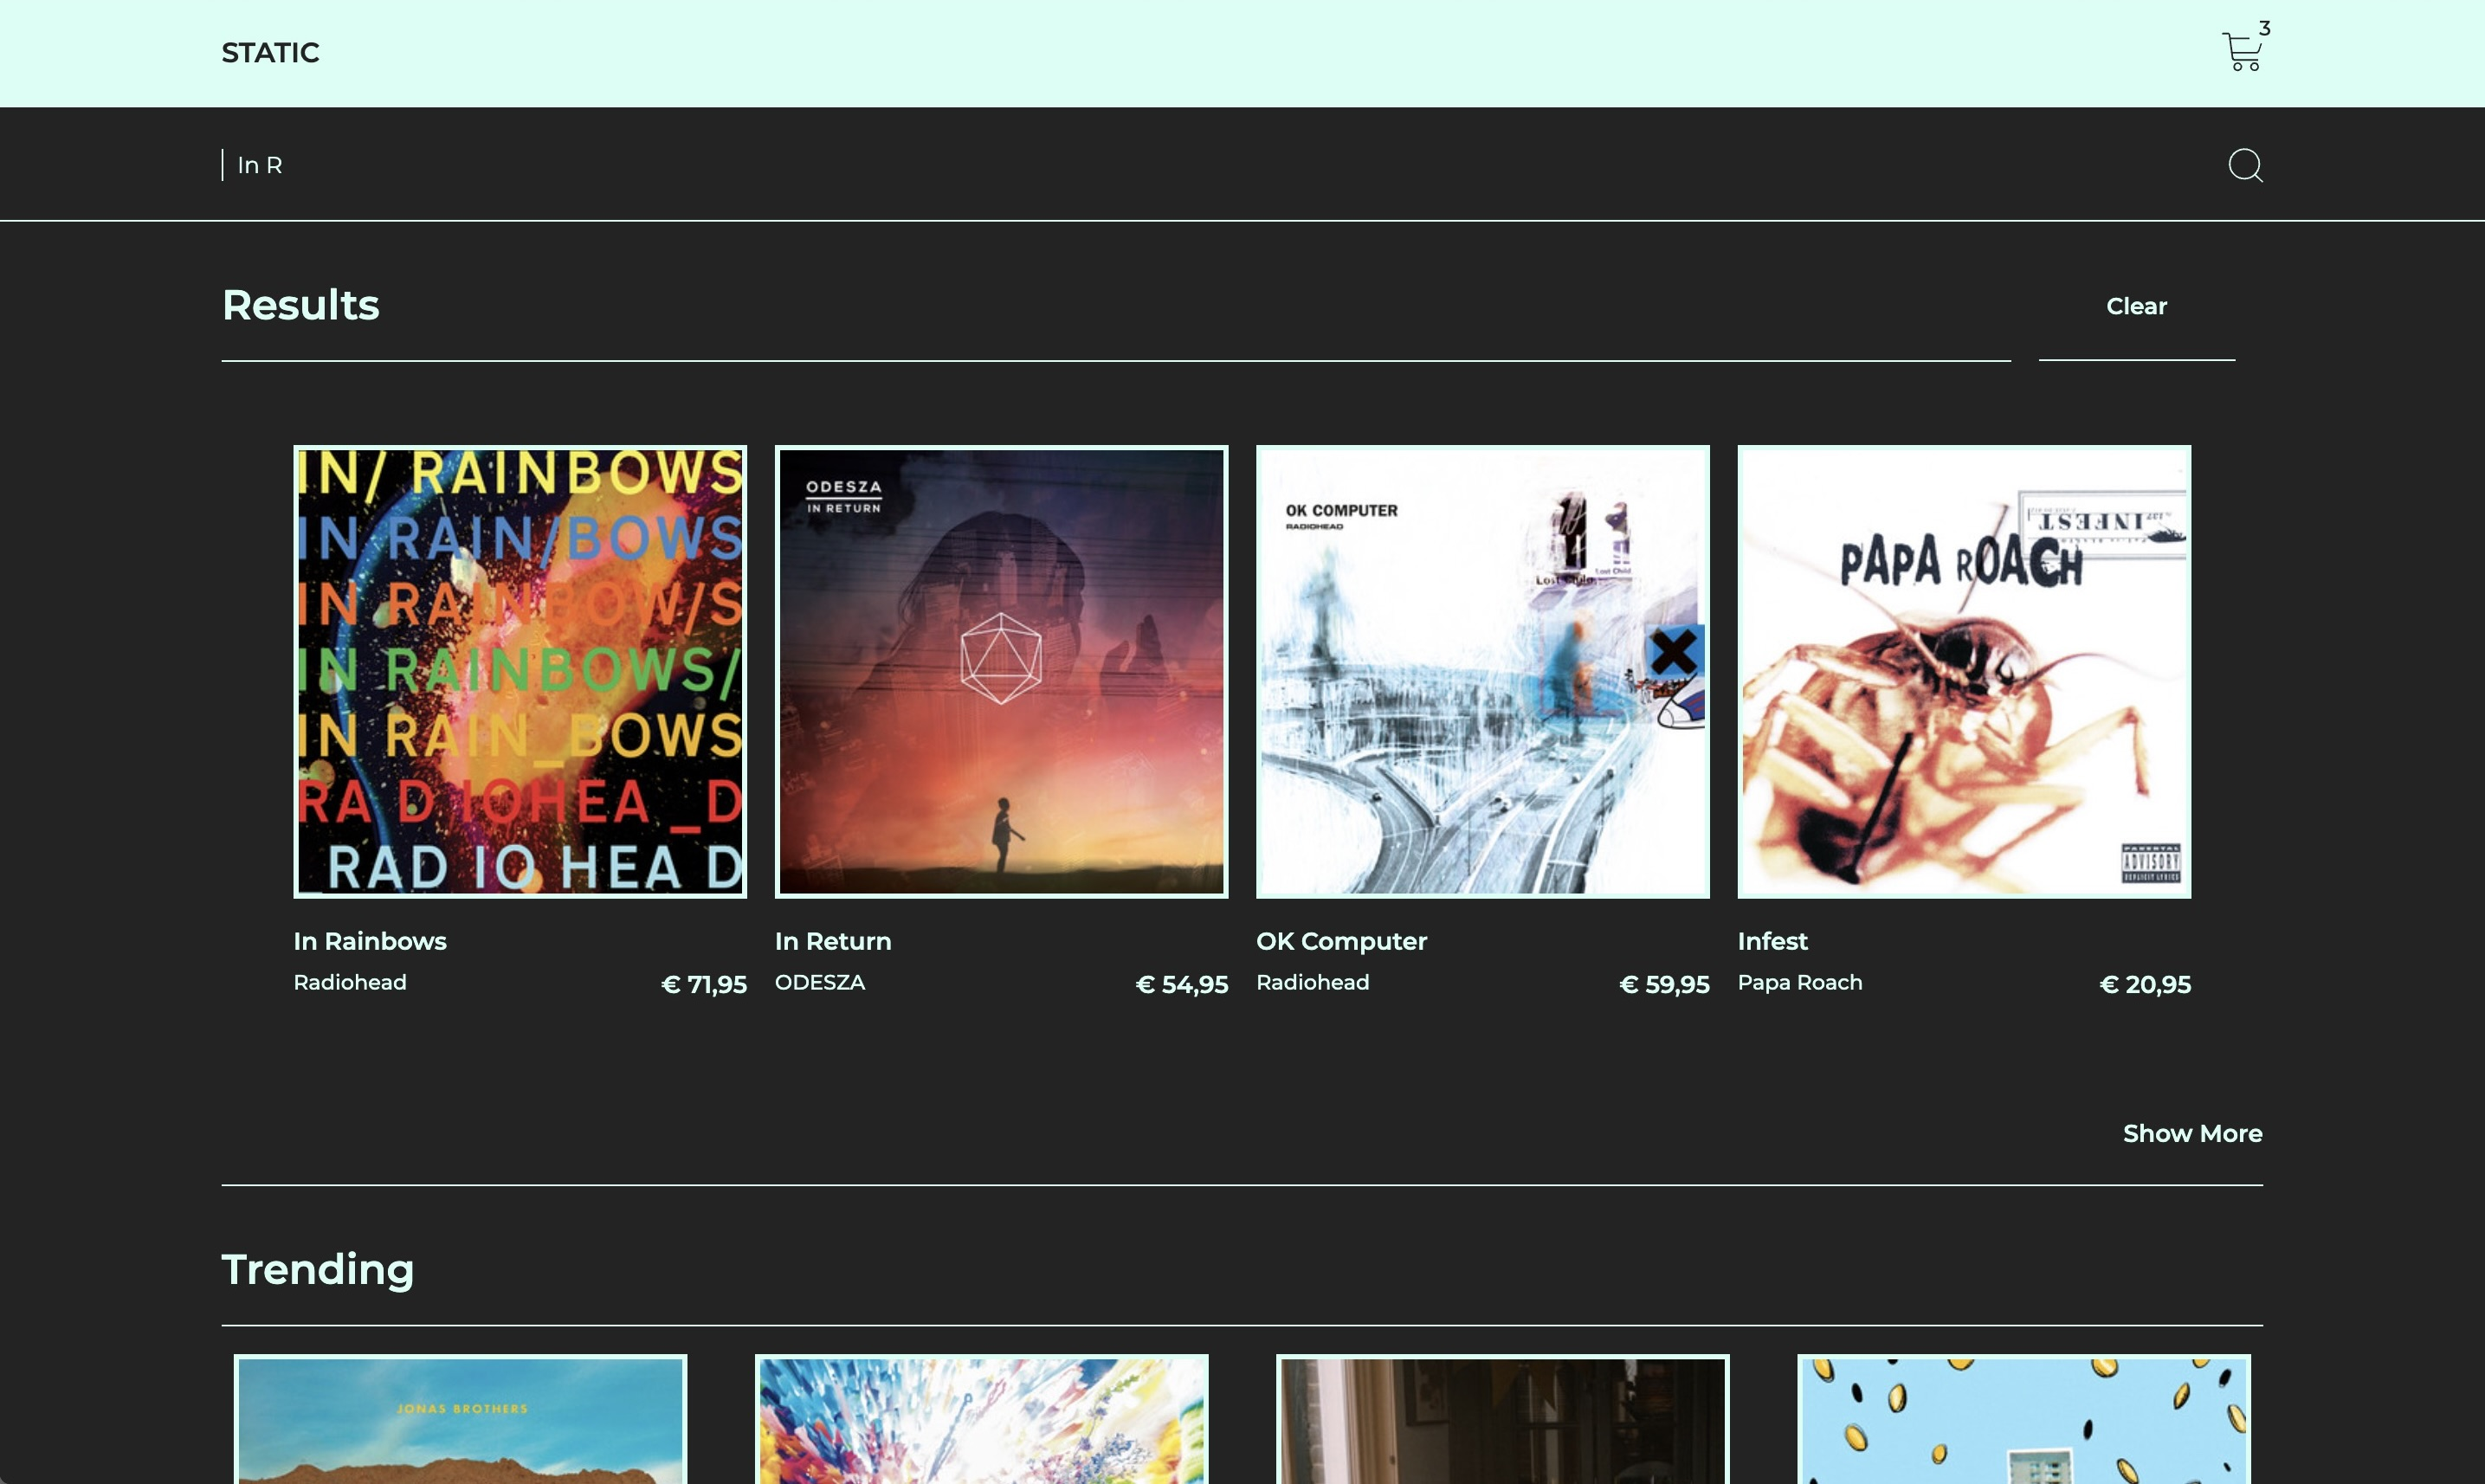
\includegraphics[width=1\linewidth]{graphics/desktopSearch}
	\caption[Desktop search]{Desktop search}
	\label{fig:desktopSearch}
\end{figure}
